\clearpage{\pagestyle{empty}\cleardoublepage}
\chapter{Linea di produzione di Verdicchio: tensioattivi per lo spiazzamento dell'acqua in condotta}
\chaptermark{Test Linea Verdicchio}
Il giorno venerdì 12 giugno 2015 è stato effettuato il test di campo del foamer Chimec  Phoenix 6163 presso il campo SNM. Dopo l''esperienza tra il 23 e il 27 febbraio 2015 presso il pozzo CZT-2d, obiettivo primario del test è stato quello di spiazzare l'acqua dalla linea San Marco (lunghezza 13,6 km, diametro 4"), così da diminuire le cadute di pressione e favorire la produzione dei pozzi a monte.
I risultati ottenuti sono stati:
\begin{itemize}
\item acqua spiazzata: 12,74 m\ap{3}
\item tempo impiegato: 2h10m
\item pressione minima: 5,5 bar
\end{itemize}
I tempi di spiazzamento, estremamente brevi, sono collegati al comportamento del foamer. Grazie alla conformazione della mandata e  alla miscela con acqua, il tensioattivo ha agito come un "pig" chimico, capace di spiazzare l'acqua dalla condotta con conseguente guadagno in termine di tempo e praticità.

\section{Impianti e giacimenti}
\subsection{Polo produttivo di San Giorgio Mare}
\subsection{Descrizione delle aree pozzo interessate}
\subsubsection{Verdicchio}
\subsubsection{San Marco}
\subsection{La centrale di San Giorgio Mare}
\subsubsection{Sala controllo}
\subsubsection{Separatori}
\subsubsection{Compressori}
\subsubsection{Pompe dosatrici}
\subsubsection{Unità di refrigerazione}
\subsubsection{Riscaldatori}
\subsection{La linea verdicchio}

\section{Configurazione sperimentale: materiali e modalità di esecuzione}
\sectionmark{Configurazione sperimentale}
\subsection{Schiumogeno}
Il prodotto CHIMEC Phoenix 8161 è un antischiuma che favorisce l'avanzamento della schiuma a valle del separatore, con conseguenze decisamente negative sull'impianto.
\subsection{Antischiumogeno}
Il prodotto CHIMEX Phoenix 6163 è uno schiumogeno; disciolto in acqua, fa diminuire notevolmente la tensione interfacciale che compete alla superficie di separazione fra la soluzione diluita così ottenuta e la fase gassosa.

\begin{figure}[ht] %%% Immagine pompa dosatrice
    \centering
    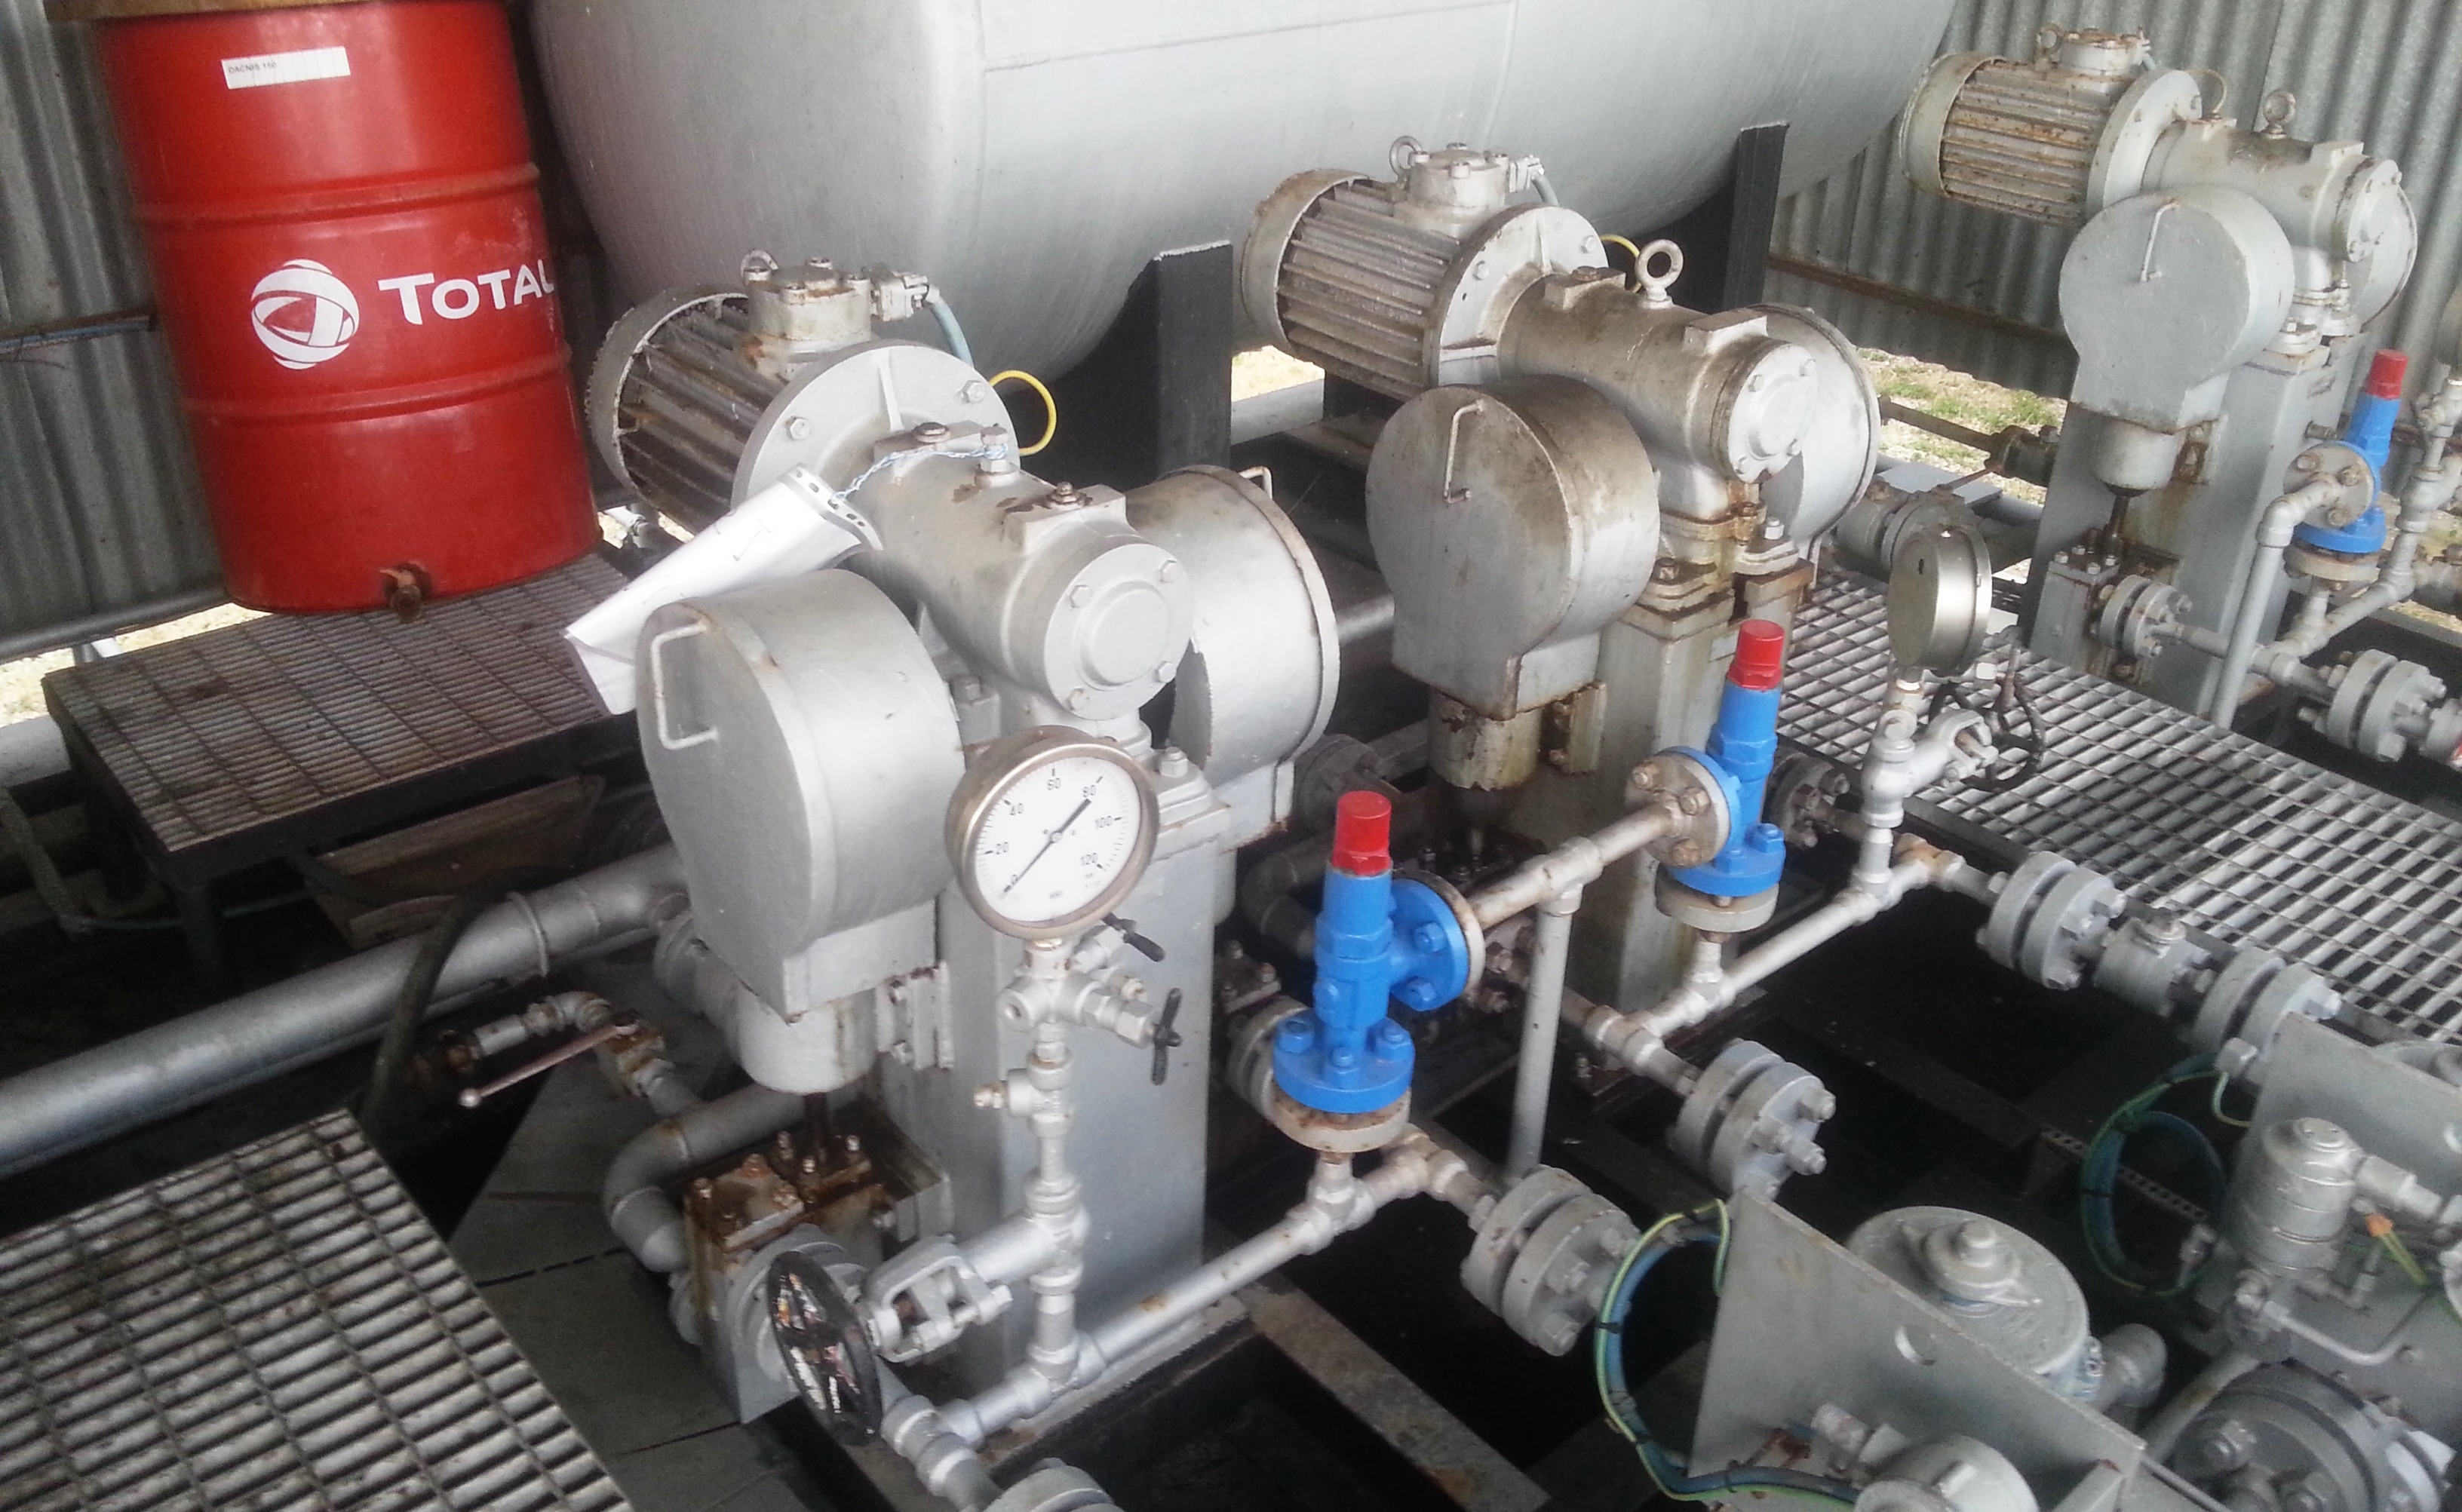
\includegraphics[width=\textwidth]{fig/test/defoamerpump.jpg}
    \caption{Pompe dosatrici impiegate per l'iniezione di defoamer a monte del separatore.} 
    \label{fig:defoamerpump}
\end{figure}

\subsection{Punto di iniezione - San Marco}

\begin{figure}[!htbp] %Immagine layout di mandata
    \centering
    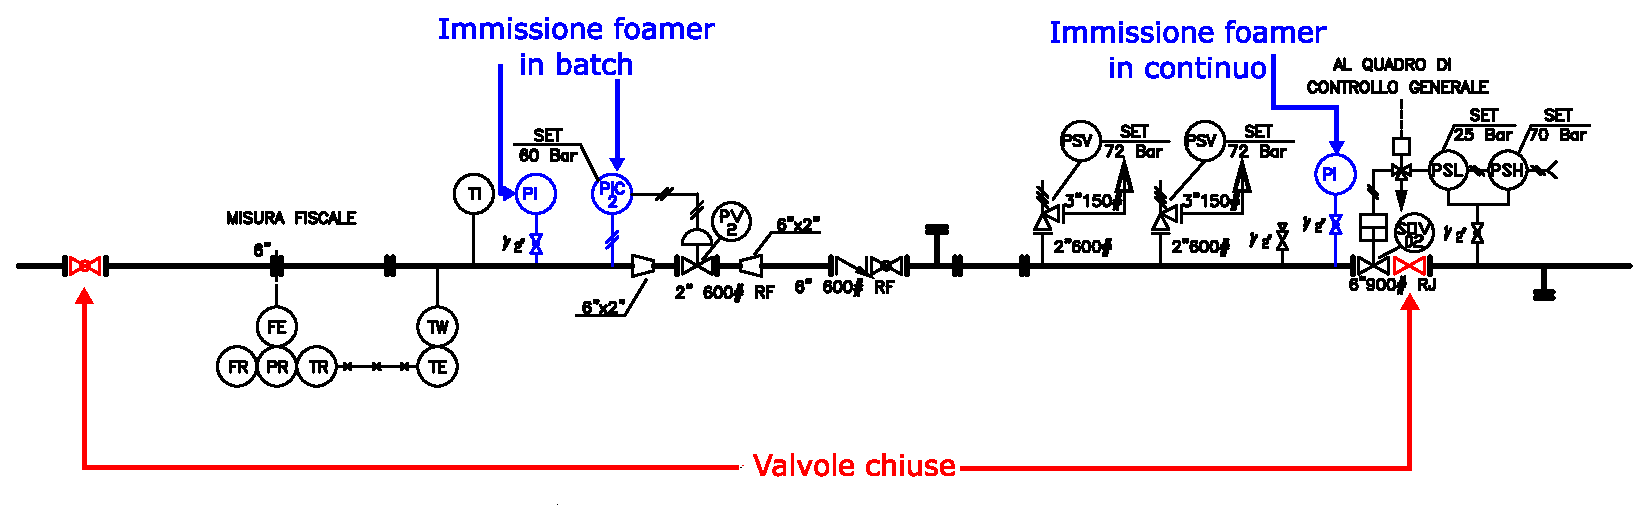
\includegraphics[width=\textwidth]{fig/test/mandata.eps}
    \caption{Layout linea di mandata SNM, modalità di applicazione del batch.} 
    \label{fig:mandata}
\end{figure}

\subsection{Apparati di misura}
\subsection{Iniezione in-batch}
\subsection{Iniezione in continuo}

I parametri di pressione e temperatura sono stati monitorati tramite un termomanometro digitale installato sulla linea di mandata, tra la Fisher e le valvole di blow-down, in corrispondenza dei due spool flangiati. Il defoamer è stato iniettato all'ingresso del separatore con una portata di 30 litri orari, in continuo, tramite l'utilizzo di pompe dosatrici già presenti alla centrale SGM ((\figurename~\ref{fig:defoamerpump}).

\section{Risultati e discussione}
\subsection{Studio degli effetti a breve termine}
\subsection{Andamento produttivo post-test}
\subsection{Analisi costi e benefici}
\subsection{Pigaggio della linea di produzione}